\documentclass{beamer}
\usepackage[utf8]{inputenc}
\usepackage{pifont}
\usetheme{Madrid}
\usecolortheme{default}

%------------------------------------------------------------
%This block of code defines the information to appear in the
%Title page
\title[Power Analysis Side-channel Attacks] %optional
{Side-channel security of superscalar CPUs}

\subtitle{}

\author[Federico Zanca] % (optional)
{Federico Zanca}

\institute[] % (optional)
{
  %\inst{1}%
  Computer Science and Engineering\\
  Politecnico di Milano
  %\and
  %\inst{2}%
  %Faculty of Chemistry\\
  %Very Famous University
}

\date[2025] % (optional)
{}

%\logo{\includegraphics[height=1cm]{overleaf-logo}}

%End of title page configuration block
%------------------------------------------------------------



%------------------------------------------------------------
%The next block of commands puts the table of contents at the 
%beginning of each section and highlights the current section:

\AtBeginSection[]
{
  \begin{frame}
    \frametitle{Table of Contents}
    \tableofcontents[currentsection]
  \end{frame}
}
%------------------------------------------------------------


\begin{document}

%The next statement creates the title page.
\frame{\titlepage}


%---------------------------------------------------------
%This block of code is for the table of contents after
%the title page
\begin{frame}
\frametitle{Table of Contents}
\tableofcontents
\end{frame}
%---------------------------------------------------------







\section{Introduction \& Context}

%---------------------------------------------------------
%Changing visivility of the text
% slide 1
%\begin{frame}
%\frametitle{The Evolving Target: Complex CPUs}
%\begin{block}{Remark}

%\end{block}

%\begin{itemize}
%    \item<1-> Text visible on slide 1
%    \item<2-> Text visible on slide 2
%    \item<3> Text visible on slides 3
%    \item<4-> Text visible on slide 4
%\end{itemize}
%\end{frame}


\begin{frame}
    \frametitle{Recap: What are Side-Channel Attacks?}
    \begin{block}{Definition}
        \begin{itemize}
            \item Side-Channel Attacks (SCAs) exploit unintended physical emanations (e.g., power consumption, electromagnetic radiation, execution time) from a device
            \item These emanations are correlated with the secret data being processed, allowing an attacker to infer sensitive information (e.g., cryptographic keys)
        \end{itemize}
    \end{block}

    \begin{block}{The Fundamental Question }
        \begin{itemize}
            \item How do we accurately \textit{model} these physical emanations to find the leaked information?
            %\item This presentation delves into the specifics of leakage modeling, especially on modern, complex CPUs.
        \end{itemize}
    \end{block}
\end{frame}
%---------------------------------------------------------
%---------------------------------------------------------
\begin{frame}
    \frametitle{Complex CPU Targets}
    \begin{block}{SCA Challenges on Modern CPUs}
    \begin{itemize}
        \item SCAs are increasingly targeting complex platforms:
            \begin{itemize}
                \item SCA targets have evolved from simple micro-controllers and smart-cards to complex single-core and laptop-grade CPUs
                \item Now, side-channel attacks are also relevant for superscalar CPUs
            \end{itemize}
        \item Assessing vulnerability and validating countermeasures becomes significantly more difficult with increasing target complexity
    \end{itemize}
    \end{block}
\end{frame}


\begin{frame}
    \frametitle{Why Microarchitecture Matters for SCA}
    \begin{block}{Main Idea} 
        \begin{itemize}
            \item To assess the side-channel vulnerability of software on a CPU, we \textbf{must} consider the CPU's microarchitectural features.
            \item Correct execution only requires the object code to match the CPU at ISA level.
            \item However, the extent of side-channel leakage also depends on the processor's microarchitecture.
        \end{itemize}
    \end{block}
\end{frame}

\begin{frame}
    \frametitle{Why Microarchitecture Matters for SCA}
    \begin{block}{Dangers of Ignoring Microarchitecture}
        \begin{itemize}
            \item Side-channel countermeasures, if designed without microarchitectural awareness, can be invalidated.
            \item \textbf{Example}: Accidental value combinations due to register reuse, despite careful assembly implementations.
        \end{itemize}
    \end{block}
\end{frame}
%---------------------------------------------------------

%---------------------------------------------------------


\section{Uncovering Microarchitecture via CPI Analysis}






\begin{frame}
    \frametitle{Uncovering Microarchitecture via CPI Analysis}
    \begin{block}{Problem: Hidden Microarchitecture}
        \begin{itemize}
            \item Internal details of CPU microarchitectures (e.g., pipelines, execution units, buffers) are often proprietary and not publicly documented in full detail.
            \item However, precise knowledge of these details is what allows mounting an effective side-channel attack
        \end{itemize}
    \end{block}
\end{frame}

\begin{frame}
    \frametitle{Uncovering Microarchitecture via CPI Analysis}
    \begin{block}{Inferring from CPI}
        \begin{itemize}
            \item A novel method is proposed: using information leaked by the \textbf{Clock cycles Per Instruction (CPI)} achieved on specific instruction sequences.
            \item \textbf{How it works}:
                \begin{itemize}
                    \item Compare CPI of instruction sequences with and without \textit{Read-After-Write (RAW) hazards}.
                    \item Hazard-free sequences reveal best-case CPU capabilities (e.g., dual-issuing).
                    \item Hazard-affected sequences show how hazards prevent parallel execution.
                \end{itemize}
            \item \textbf{Key Interpretations:}
                \begin{itemize}
                    \item A CPI of \textbf{0.5} indicates \textbf{full dual-issuing} (2 instructions per cycle).
                    \item A sustained CPI of \textbf{1} implies a component is \textbf{fully pipelined} (can start a new operation every cycle).
                \end{itemize}
        \end{itemize}
    \end{block}
\end{frame}

\begin{frame}
    \frametitle{Example: ARM Cortex-A7 MPCore}
    \begin{block}{CPU Overview}
        \begin{itemize}
            \item A dual-core, in-order CPU with an 8-stage pipeline.
            \item Described as "partial dual-issue": Not all instruction pairs can be executed simultaneously.
        \end{itemize}
    \end{block}

    \begin{block}{Why Characterize This CPU?}
        \begin{itemize}
            \item Public documentation (reference manuals, GCC backend descriptions) provides a logical view (see next slide).
            \item However, it lacks some microarchitectural details needed for side-channel analysis
        \end{itemize}
    \end{block}
\end{frame}


\begin{frame}
    \frametitle{ARM Cortex-A7 Pipeline Logical View}
    \begin{figure}
        \centering
        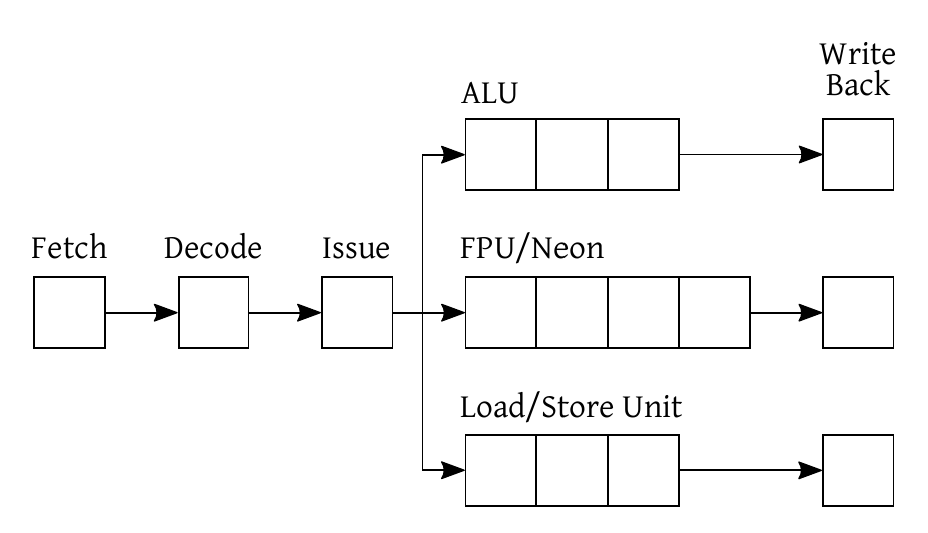
\includegraphics[width=0.8\textwidth]{Pictures/cortexA7.png} 
        \caption{ARM Cortex-A7 MPcore pipeline logical view }
        \label{fig:cortex-a7-pipeline}
    \end{figure}
\end{frame}


\begin{frame}
    \frametitle{Undercovering Microarchitectures (Cortex-A7 Example)}
    \begin{block}{Inferences from CPI Analysis}
        \begin{itemize}
            \item \textbf{ALUs:} Two ALUs are present, but they are not identical. Only one is equipped with a barrel shifter and multiplication unit.
            \item \textbf{Pipelined Units:}
                \begin{itemize}
                    \item The \textbf{Load Store Unit (LSU)} is \textbf{fully pipelined} (sustained CPI of 1 for load/store sequences).
                    \item The \textbf{multiplier} within the ALU is also \textbf{fully pipelined} (CPI of 1 for multiplication sequences).
                \end{itemize}
            \item \textbf{Data Bus Structure:}
                \begin{itemize}
                    \item Three data buses connect the Register File (RF) to the Execution (EX) stage.
                    \item Two buses connect the EX stage back to the RF, implying the RF has two write-ports and three read-ports.
                \end{itemize}
            \item \textbf{Unexpected NOP Behavior:} Counter-intuitively, \texttt{nop} instructions are \textbf{not dual-issued} by the Cortex-A7.
        \end{itemize}
    \end{block}
\end{frame}



\begin{frame}
    \frametitle{Deduction: Cortex-A7 Pipeline Structure}
    \begin{figure}
        \centering
        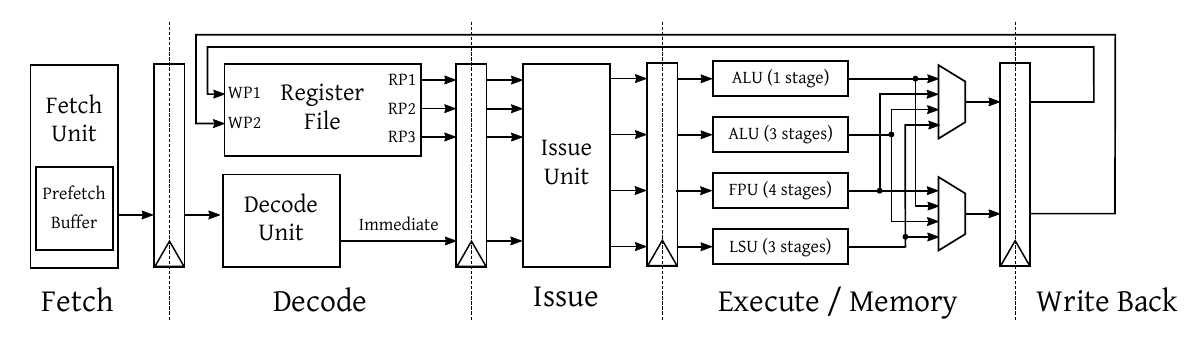
\includegraphics[width=1.0\textwidth]{Pictures/cortexUncovered.png}
        \caption{Alleged ARM Cortex-A7 pipeline structure according to CPI analysis deductions }
        \label{fig:deduced-pipeline}
    \end{figure}
\end{frame}



\begin{frame}
    \frametitle{Dual-Issue Capabilities: Instruction Pairs}
    \begin{table}
        \centering
        \small % makes the content of the table smaller
        \caption{Instruction pairs executed in dual-issue by the Cortex-A7 MPCore CPU. }
        \label{tab:dual-issue-pairs}
        \begin{tabular}{|l|c|c|c|c|c|c|c|}
            \hline
            \textbf{} & \textbf{mov} & \textbf{ALU} & \textbf{ALU w/imm} & \textbf{mul} & \textbf{shifts} & \textbf{branch} & \textbf{ld/st} \\
            \hline
            \textbf{mov}        & \checkmark & \checkmark & \checkmark & \ding{55} & \checkmark & \checkmark & \ding{55} \\
            \textbf{ALU}        & \checkmark & \ding{55}  & \checkmark & \ding{55} & \ding{55}  & \checkmark & \ding{55} \\
            \textbf{ALU w/ imm} & \checkmark & \checkmark & \checkmark & \ding{55} & \checkmark & \checkmark & \checkmark \\
            \textbf{branch}     & \checkmark & \checkmark & \checkmark & \checkmark & \checkmark & \ding{55}  & \checkmark \\
            \textbf{ld/st}      & \checkmark & \ding{55}  & \checkmark & \ding{55} & \ding{55}  & \checkmark & \ding{55} \\
            \textbf{mul}        & \ding{55}  & \ding{55}  & \ding{55}  & \ding{55} & \ding{55}  & \checkmark & \ding{55} \\
            \textbf{shifts}     & \ding{55}  & \ding{55}  & \checkmark & \ding{55} & \ding{55}  & \checkmark & \ding{55} \\
            \hline
        \end{tabular}
    \end{table}
\end{frame}
\section{SCA Characterization \& Leakage Modeling}

\begin{frame}
    \frametitle{Characterizing Microarchitecture Leakage}
    \begin{block}{The Foundation of Leakage}
        \begin{itemize}
            \item Gates driving large capacitive loads are primary sources of side-channel leakage.
            \item Power consumption in such scenarios is well-modeled by the \textbf{Hamming distance} of two values asserted on their outputs in subsequent clock cycles
        \end{itemize}   
    \end{block}

    \begin{block}{Detecting Leakage}
        \begin{itemize}
            \item \textbf{Pearson's correlation coefficient} is used to statistically compare measured power consumption with the predicted leakage model
            \item A correlation statistically distinguishable from zero (with >99.5\% confidence) in the correct clock cycle indicates a leakage
        \end{itemize}
    \end{block}
\end{frame}


\begin{frame}
    \frametitle{Leakage Measurement - Cortex-A7}
    \begin{block}{Data Collection}
        \begin{itemize}
            \item Seven micro-benchmarks: small (2-4) instruction sequences designed to trigger specific component activities
            \item Ran with randomly generated values at each execution, triggered by GPIO
            \item Cache effects eliminated by measuring executions after the first one and inserting 100 \texttt{nop}s
            \item Data acquired: \textbf{100,000 power traces} per benchmark
            \item Each trace was an average of 16 individual executions with the same input, reducing noise
            \item Register File (RF) leakage was evaluated separately by pre-charging destination registers
        \end{itemize}
    \end{block}
\end{frame}

%------------------------------------------------------

\begin{frame}
    \frametitle{Observed Leakage: Registers}
    \begin{block}{Register File (RF)}
        \begin{itemize}
            \item No statistically significant leakage observed from RF read-ports.
            \item Attributed to a short capacitive load, as Issue Stage (IS) buffers drive execution units
        \end{itemize}
    \end{block}
\end{frame}

\begin{frame}
    \frametitle{Observed Leakage: IS/EX}
    \begin{block}{Issue/Execution (IS/EX) Buffers}
        \begin{itemize}
            \item Outputs show significant leakage
            \item \textbf{Modeled by Hamming Distance:} between values of a source operand of an older and a younger single-issued instruction
                \begin{itemize}
                    \item Leakage prominent when operands share the same bus (same source operand position)
                \end{itemize}
            \item \textbf{Hamming Weight Leakage:} Also observed when \texttt{mov}s are interleaved with \texttt{nop}s (due to \texttt{nop} implementation with zero-valued operands)
            \item Dual-issued arithmetic instructions show no measurable leakage among source operands (no shared resources before computation)
        \end{itemize}
    \end{block}
\end{frame}



\begin{frame}
    \frametitle{Observed Leakage: ALUs }
    \begin{block}{ALU and Shift Buffer}
        \begin{itemize}
            \item \textbf{ALU:} Leakage dependent on the \textbf{Hamming weight} of the instruction result
                \begin{itemize}
                    \item Inferred due to ALUs asserting results on previously zero-precharged signals
                \end{itemize}
            \item \textbf{Shift Buffer:} A small leakage proportional to the \textbf{Hamming weight} of the shifted value is present
        \end{itemize}
    \end{block}
\end{frame}

\begin{frame}
    \frametitle{Observed Leakage: EX/WB Buffers}
    \begin{block}{Execution/Write-Back (EX/WB) Buffers}
        \begin{itemize}
            \item Leakage mirrors IS/EX buffers.
            \item \textbf{Modeled by Hamming Distance:} between the \textit{results} of subsequent single-issued instructions.
                \begin{itemize}
                    \item Occurs regardless of destination register sharing or data-flow relationship
                \end{itemize}
            \item \textbf{Hamming Weight Leakage:} Also present for instruction results.
                \begin{itemize}
                    \item Attributed to \texttt{nop} instructions resetting the WB bus to zero 
                \end{itemize}
        \end{itemize}
    \end{block}
\end{frame}




\begin{frame}
    \frametitle{Observed Leakage: MDR}
    \begin{block}{Memory Data Register (MDR) and Align Buffer}
        \begin{itemize}
            \item Potential leakage source during load/store instruction sequences
            \item \textbf{Modeled by Hamming Distance:} between two subsequently loaded or stored values
            %\item Applies even to half-word and single-byte loads/stores (power proportional to HD between full 32-bit words).
            \item Suggests a separate buffer in the Load Store Unit (LSU) for sub-word realignment
            \item Presence of this \textbf{align buffer} and its leakage was confirmed experimentally
        \end{itemize}
    \end{block}
\end{frame}


\begin{frame}
    \frametitle{Superscalar Leakage Modeling}
    \begin{block}{Leakage from Algorithmically Independent Instructions}
        \begin{itemize}
            \item Observed information leakage that combines values from potentially independent instructions, driven by four causes:
                \begin{enumerate}
                    \item Instruction scheduling order
                    \item Position of source operands
                    \item Single or dual-issuing of instructions
                    \item Potential data remanence in LSU buffers
                \end{enumerate}
        \end{itemize}
    \end{block}
\end{frame}
\begin{frame}
    \frametitle{Superscalar Leakage Modeling}
    \begin{block}{Subtle Code Changes can be Harmful}
        \begin{itemize}
            \item Even apparently harmless changes to assembly code (e.g., swapping source operands of a commutative operation like XOR) can lead to side-channel leakage
            \item This is due to altered pipeline resource sharing
            \item Such changes are difficult to detect by tools focusing only on instruction semantics or manual audits
        \end{itemize}
    \end{block}
\end{frame}




\begin{frame}
    \frametitle{Superscalar Leakage: Vulnerabilities}
    \begin{block}{Impact of Dual-Issuing}
        \begin{itemize}
            \item Worsens effects of instruction scheduling and operand position.
            \item Leakage can stem from combinations of source operands of \textit{non-consecutive} instructions if an intermediate instruction is dual-issued
            \item Highlights the crucial, often-neglected importance of instruction scheduling for preventing side-channel leakage
            \item Dual-issuing could also potentially \textbf{enhance security} by enabling parallel computation of two shares in masking schemes
        \end{itemize}
    \end{block}
\end{frame}
\begin{frame}
\frametitle{Superscalar Leakage: Vulnerabilities}
    \begin{block}{Data Remanence and NOPs}
        \begin{itemize}
            \item \textbf{Data Remanence:} In MDR and LSU buffers, old data can accidentally combine with current computation results, creating harmful leakage.
            \item \textbf{NOP Operations:} While semantically neutral, \texttt{nop} instructions can introduce new leakage modes (e.g., by resetting buses to zero). They are not \textit{security neutral}
        \end{itemize}
    \end{block}
\end{frame}





\end{document}